\spaltenanfang

Es gab eine Zeit, in der es keine Computer gab. Danach kam eine Zeit, in der der Zugang zu Computern ein Privileg war. Dann kam das Internet; doch es war w\"ust und leer. Sp\"ater wurde das Internet zwar gr\"o{\ss}er, aber man konnte es nur von Computern erreichen, die fest an Schreibtischen standen.

Aber schon viel viel fr\"uher gab es Bibliotheken, Orte an denen Wissen gelagert wurde, mit geheimen Priesterschaften und obskuren Referenzsystemen. Diese fast magischen Orte gibt es heute immer noch.

Und f\"ur jeden kommt die Zeit im Studium, zu der das Internet nicht mehr ausreicht, um Forschung zu betreiben. Vielleicht will man ja auch nur ungest\"ort lernen, das Internet geht grad nicht oder die Aufbereitung von Informationen in B\"uchern liegt einem einfach mehr. Dann sollte man in eine Bibliothek gehen.

Und von denen gibt es nat\"urlich mehrere.\\
Die \textbf{Institusbibliothek Informatik} ist direkt \"uber dem Lernzentrum.
Sie ist vor allem auf Fachliteratur zur Informatik spezialisiert (obwohl wir von
mindestens einem Buch wissen, das definitv Science Fiction ist). Von Handb\"uchern und
Softwarereferenzen zu den Lieblingsb\"uchern der Professoren findet man dort
einiges, was einem im Studium weiterhelfen kann. Manche Tagungsb\"ande sind aber nicht in der Bibliothek selbst,
sondern in Magazinen tief unter dem Institut (tiefer als das Rechenzentrum im Keller), so dass man einen Mitarbeiter losschicken muss, wenn man ein entsprechendes Buch braucht.\\
Die \textbf{Bereichsbibliothek der Mathematik} ist unter dem Dach auf der anderen Stra{\ss}enseite. Wer viel Mathe macht, wird da fr\"uher oder sp\"ater mal vorbeikommen.\\
Die \textbf{Universit\"atsbibliothek} ist auch in Bockenheim, auf der anderen Seite der Bockenheimer Warte. Dort findet man auch Archive von Fachzeitschriften und vieles mehr.\\
Nat\"urlich gibt es auf den anderen Campus noch mehr gro{\ss}e und kleine Bibliotheken, wie z.B. die \textbf{Naturwissenschaftliche Bibliothek} am Campus Riedberg im Otto-Stern-Zentrum. Und am Campus Westend gibt es natürlich auch einige Bibliotheken.

Je nachdem, was ihr studiert, solltet ihr die Studenten aus dem entsprechenden Fachbereich fragen, wo dessen Bibliotheken zu finden sind.

\begin{center}
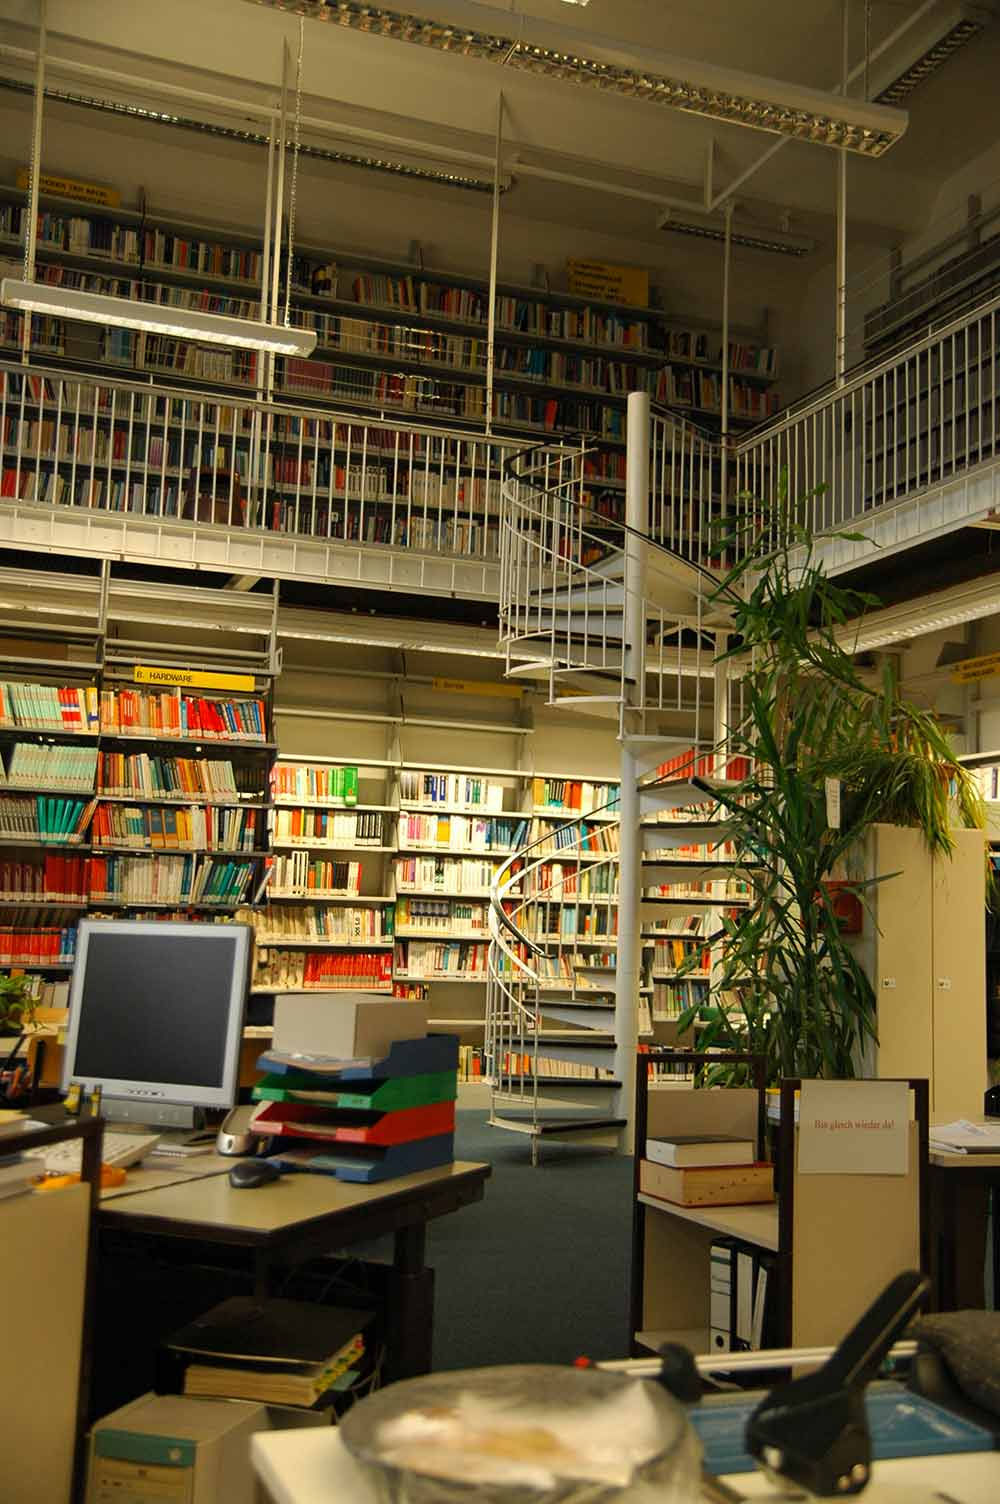
\includegraphics[width=0.7\linewidth]{bilder/bib.jpg}
\end{center}

Na dann viel Spass beim Lesen.
\spaltenende
